\section{Sistemas de reconhecimento de caracteres}
Segundo \cite{silva2003reconhecimento}, os sistemas de reconhecimento ótico de caracteres são sistemas desenvolvidos para, de certa forma, reproduzir a capacidade humana de ler textos.

	\subsection{Origens e Evolução}
	\cite{man1986pattern} disse que as origens da tentativa de sumular a leitura humana datam de 1870, quando foi inventado por Carey, o scanner de retina. A partir da evolução dos dispositivos capazes de captar e traduzir imagens em sinais que podiam ser medidos, novos horizontes foram descobertos. Entretanto, a primeira tentativa bem sucedida de reconhecimento de caracteres foi realizada somente em 1990 pelo cientista russo Tyutin, que desenvolveu um sistema que visava o auxílio de deficientes visuais.
	
	Alguns dos motivos do desenvolvimento de um sistema de reconhecimento de caracteres são:
	\begin{itemize}
		\item Aquisição de dados numéricos comerciais;
		\item Compactação de dados;
		\item Leitura automática de formulários;
		\item Identificação de endereçamento postal;
		\item Reconhecimento de cheques bancários;
		\item Sistemas de aquisição de textos para a tradução automática;
		\item Interface homem x máquina mais natural e sem necessidade de recodificação dos dados (sujeitos a um menor número de erros, pois não é necessário redigitar os textos, introduzindo novos erros);
		\item Auxílio a deficientes visuais, na leitura de textos (tradução e impressão automática em braile)
	\end{itemize}

	\subsection{Tipos de Sistemas de Reconhecimento de Caracteres}
	Os sistemas de reconhecimento de caracteres podem ser desenvolvidos utilizando-se diferentes procedimentos tanto de aquisição de dados como de processamento de informações além de serem orientados para diferentes tipos de aplicações.
	
	Podem ser classificados primeiramente quanto ao tipo de mecanismo utilizado na aquisição dos textos a serem reconhecidos. Nesta categoria, encontram-se os sistemas magnéticos, sistemas mecânicos e sistemas óticos.
	
	Dentro dos sistemas OCR, são encontradas duas classes importantes, aqueles que são baseados no processamento sequencial das informações e os baseados no processamento paralelo. Existem três categorias princiapais: sistema de reconhecimento online, sistema de reconhecimento de caracteres isolados e sistema de reconhecimento de escrito cursiva.
	
	\begin{figure}[!htb]
		\centering
		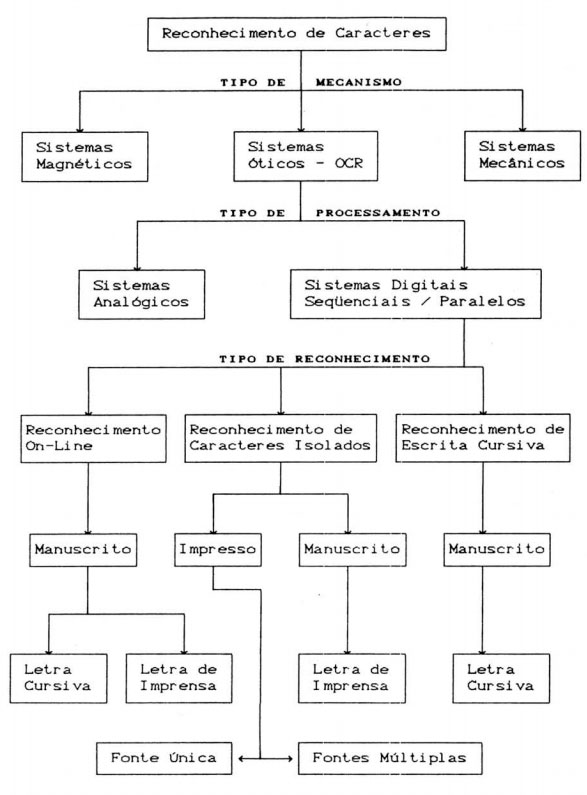
\includegraphics[scale=0.4]{img/organograma-tipos.jpg}
		\caption{Organograma}
		\label{Organograma}
	\end{figure}
	
	\subsection{Descrição dos Sistemas OCR}
	Existem diferentes etapas de processamento das informações visando o reconhecimento de textos por um sistema OCR. Estas etapas se estendem desde a captura da imagem do texto até a obtenção final de uma identificação deste. Em um sistema de COR não se deve considerar apenas a parte referente às técnicas empregadas na resolução do problema de classificação, mas um item de extrema importância é a medicação e avaliação dos resultados obtidos por estes.
		\subsubsection{Etapas de Processamento}
		Em geral, os sistemas de OCR possuem implementadas as seguintes funções: aquisição da imagem do texto, tratamento da imagem, localização e separação dos caracteres, pré-processamento dos padrões, extração de atributos, reconhecimento/classificação dos padrões e pós-processamento.
		
		\begin{figure}[!htb]
			\centering
			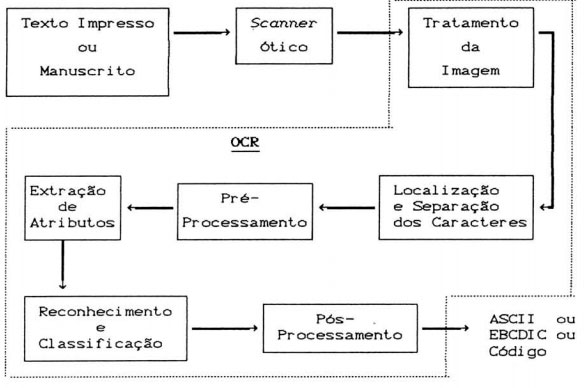
\includegraphics[scale=0.5]{img/etapas-de-processamento.jpg}
			\caption{Etapas do processo de reconhecimento}
			\label{Etapas do processo de reconhecimento}
		\end{figure}
		
		Para a separação dos caracteres, o algoritmo tem que levar em consideração diversos fatores, entre eles: o espaçamento entre caracteres e tamanho do caractere (fixo ou variável), a utilização de uma grade auxiliar (no caso de formulários com espaçamento bem definidos), e o tipo de texto a ser reconhecido, onde podem haver caracteres que se tocam ou caracteres com descontinuidade (características muito importante para módulos de segmentação). Esta etapa de processamento é até hoje uma das etapas mais críticas, sendo um problema ainda não completamente solucionado.
		
		Após terem sido isolados os caracteres, e preferencialmente, com a realização de um ajuste de tamanho e posição pré-definidos, pode-se então realizar uma etapa de extração de atributos. Esta etapada é opcional e dependerá exclusivamente do tipo de técnica empregada no reconhecimento e classificação dos padrões.
		
		\subsubsection{Técnicas de Reconhecimento}
		Existem diferentes técnicas empregadas no reconhecimento de padrões, mas estas podem ser classificadas em três grandes categorias, técnicas baseadas em:
		\begin{itemize}
			\item Atributos globais
			\item Distribuição de pontos e atributos geométricos
			\item Topológicos
		\end{itemize}